\documentclass{article}

\author{Michael Cardiff}
\date{\today}

%% science symbols
\usepackage{amsmath,amssymb,amsthm}  % ams
\usepackage{siunitx}
\usepackage{bm,cancel}               % look nice
\usepackage{physics,slashed}         % phys specific

%% general pretty stuff
\usepackage{caption,float,graphicx,url,enumitem}
\usepackage{tikz,tikz-feynhand}
\usepackage{geometry}
\usepackage{booktabs}

% setup options
\captionsetup{labelfont=bf}
\geometry{margin=1in}

% macros
\renewcommand{\L}{\mathcal{L}}
\renewcommand{\H}{\mathcal{H}}
\renewcommand{\bar}{\overline}
\renewcommand{\l}{\ell}
\newcommand{\id}{\bm{1}}
\newcommand{\mcV}{\mathcal{V}}
\newcommand{\D}{\partial}
\newcommand{\M}{\mathcal{M}}
\newcommand{\veps}{\varepsilon}
\newcommand{\circled}[1]{\tikz[baseline=(char.base)]{
    \node[shape=circle,draw,inner sep=2pt](char){#1};}}

% mdframed environments
\usepackage[framemethod=TikZ]{mdframed}
\mdfsetup{skipabove=\topskip,skipbelow=\topskip}
\mdfdefinestyle{defstyle}{%
  linewidth=1pt,
  frametitlerule=true,
  frametitlebackgroundcolor=gray!40,
  backgroundcolor=gray!20,
  innertopmargin=\topskip
}

\mdfdefinestyle{todostyle}{%
  linewidth=0pt,
  frametitlerule=false,
  frametitlebackgroundcolor=red!40,
  backgroundcolor=red!20,
  innertopmargin=\topskip
}

\mdtheorem[style=defstyle]{definition}{Definition}
\mdtheorem[style=defstyle]{theorem}{Theorem}
\mdtheorem[style=defstyle]{problem}{Problem}
\mdtheorem[style=defstyle]{example}{Example}

\numberwithin{example}{section}

\newenvironment{thebook}
{\begin{mdframed}[style=defstyle,frametitle={From the Book}]}{\end{mdframed}}

\newenvironment{remark}
{\begin{mdframed}[style=defstyle,frametitle={Remark}]}{\end{mdframed}}

\newenvironment{TODO}
{\begin{mdframed}[style=todostyle,frametitle={TO DO}]}{\end{mdframed}}

\theoremstyle{plain}
\newtheorem*{note}{Note}
\newtheorem*{aside}{Aside}

\title{\vspace{-3em}Particle Physics Notes}
\date{\today}

% setups
\graphicspath{ {./figs/} }

\begin{document}
\maketitle

% -*- TeX-master: "master.tex" -*-
\section{Introduction}

Two important questions in physics:
\begin{itemize}
\item What is matter made of?
  \begin{itemize}
  \item What are the elementary constituents?
  \end{itemize}
\item How do the elementary constituents interact?
  \begin{itemize}
  \item What are the forces and dynamics in Nature?
  \end{itemize}
\end{itemize}

Most popular media focus on the first question. In Fermilab's ``search for the top quark'', or the LHC ``quest for the Higgs boson'', focus is placed on the excitement of discovering new forms of matter.

This is fun, but what is really exciting is not garnering a new trophy, but in what the existance of these new particles implies for the second question --- what new dynamics must exist that this new particle can help reveal?

\subsection{The matter}
\begin{itemize}
\item Hydrogen:
  \begin{figure}[H]
    \centering
    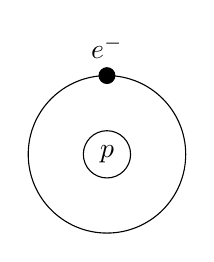
\begin{tikzpicture}{scale=1.5}
      \draw (0,0) circle [radius=0.3] node {$p$};
      \draw (0,0) circle [radius=1.0];
      \filldraw (0,1.0) circle [radius=0.1]
      node [yshift=1em] {$e^-$};
    \end{tikzpicture}
    \caption{Hydrogen Atom}
    \label{fig:hydrogen}
  \end{figure}
  A visualization is in fig~\ref{fig:hydrogen} Some properties of hydrogen:
  \begin{gather*}
    \text{Radius: } r_e\approx \SI{1}{\angstrom}\\
    \text{Binding Energy: }\SI{13}{\eV}
  \end{gather*}
  The unit of the binding energy is an Electron-Volt, which is what we will use for all energies for the duration of these notes.
  \begin{definition}[Electron-Volt]
    The electron volt is defined as the kinetic energy of an electron accelerated across a 1V potential, the usual SI unit prefixes can be applied such that 1keV=$10^3$eV, 1MeV=$10^6$eV etc.
  \end{definition}
\item Electron
  \begin{gather*}
    \text{Mass: } m_e= 0.511\text{ MeV}\\
    \text{Charge}=-1\\
    \text{Spin}=\frac12
  \end{gather*}
\item Proton
  \begin{gather*}
    \text{Mass: } m_p= 938\text{ MeV}\approx 1\text{ GeV}\\
    \text{Charge}=+1\\
    \text{Spin}=\frac12
  \end{gather*}
  \item Neutron
  \begin{gather*}
    \text{Mass: } m_n= m_p+1.3\text{ MeV}\approx m_p\\
    \text{Charge}=0\\
    \text{Spin}=\frac12
  \end{gather*}
  \item Deuterium is a Hydrogen with a neutron
\end{itemize}

\paragraph{Sizes}
\begin{itemize}
\item The electron is effectively a point
\item The nucleons, which are protons and neutrons have a ``radius'' of $\sim 10^{-15}$m, which is given the name of $1$fm, a ``Fermi'' or femtometer, which is notably less than the scale of hydrogen
\end{itemize}

\subsection{Forces in play:}
\begin{itemize}
\item Gravity $\sim$ negligible:
  \begin{align*}
    F=G_N\frac{m_p m_e}{r^2}
  \end{align*}
\item Electric:
  \begin{align*}
    F=\frac{e^2}{4\pi}\frac{Q_p Q_e}{r^2}
  \end{align*}
\item Strong --- Binds nucleons into nuclei
\item Weak --- Causes nuclear ``beta'' decay, and fusion
\end{itemize}

\subsection{Beta ($\beta$) decay}
A Process described by:
\begin{align*}
  n\to p+e^{-}+\bar{\nu}_e
\end{align*}
Where $\bar{\nu}_e$ is an anti-electron neutrino. This process has a lifetime $\tau$ of $\~14$ minutes.

Note that $m_n-m_p>m_e$

\paragraph{Q/ Why doesn't deuterium decay?} In short, conservation of energy, since $2m_p+m_e+m_{\nu_e}=1877.05$MeV, however, the mass of deuterium is $m_d=1876.64$. The masses are not large enough to allow for this decay:
\begin{figure}[H]
  \centering
  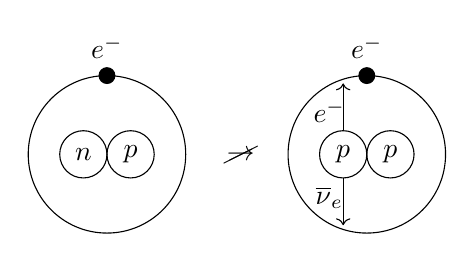
\begin{tikzpicture}
    \draw (0,0) circle [radius=0.3] node {$n$};
    \draw (0.6,0) circle [radius=0.3] node {$p$};
    \draw (0.3,0) circle [radius=1.0];
    \filldraw (0.3,1.0) circle [radius=0.1]
    node [yshift=1em] {$e^-$};
    \node at (2.0,0) {$\cancel{\rightarrow}$};
    \draw (3.3,0) circle [radius=0.3] node {$p$};
    \draw (3.9,0) circle [radius=0.3] node {$p$};
    \draw (3.6,0) circle [radius=1.0];
    \filldraw (3.6,1.0) circle [radius=0.1]
    node [yshift=1em] {$e^-$};
    \draw[->] (3.3,-0.3) to (3.3,-0.9) node [yshift=1em] {\hspace{-1em}$\bar{\nu}_e$};
    \draw[->] (3.3,0.3) to (3.3,0.9) node [yshift=-1em] {\hspace{-1em}$e^{-}$};
  \end{tikzpicture}
  \caption{Theoretical Deuterium Decay}
\end{figure}

\paragraph{Neutrinos and $\beta$ decay}
The other interesting story of $\beta$ decay is regarding the neutrino. In 1930, Chadwick observed the decay of tritium: $^3$H $\to\ ^3$He$+e^-$. Strangely, the $e^-$ was \emph{not} monoenergetic, as conservation of energy and momentum would require. This was catastrophic, and confronted with experimental evidence, many were prepared to throw out energy conservation. Pauli proposed a ``desperate remedy'' that some invisible particle must be carrying the energy away. Fermi's theory of weak interactions described this particle as a ``neutrino'' (little neutral one), and successfully described $\beta$ decay.

\textbf{Note}: The neutrino in $\beta$ decay was later found to be an antiparticle.

\begin{itemize}
\item Neutrinos then can be added to our list of ``matter''
  \begin{align*}
    \SI{0.01}{\eV}\leq m_{\nu_e}\leq\SI{1.4}{\eV}
  \end{align*}
  A consequence of this mass is that we can take neutrinos to be kinematically massless.
\end{itemize}

\subsection{Antiparticles}
Every particle has an antiparticle with opposite quantum numbers, but identical mass and spin:
\begin{itemize}
\item The electron $e^-$ has the positron $e^+$
\item The proton $p$ has the antiproton $\bar{p}$
\item The neutron $n$ has the antineutron $\bar{n}$
\item And the neutrinos $\nu$ have the antineutrinos $\bar{\nu}$ as we have seen
\end{itemize}
These (specifying the electron neutrino and its antiparticle) compose $\sim100\%$ of all the \textbf{observed} matter in the universe, though are only $5\%$ of the total matter.

Up to this point we have used chemistry and nuclear physics, particle physics picks up at the next level of depth.

\subsection{Quarks}
As it turns out, the proton and neutron are \textbf{not} fundamental.

If you perform a Rutherford-like scattering experiment at large energies (short distance), you find that protons and neutrons are composed of 3 hard spheres, called ``constituent quarks''

In fact, we go a bit deeper and find:
\begin{itemize}
\item The up quark $u$ and the up antiquark $\bar{u}$
\item The down quark $d$ and the down antiquark $\bar{d}$
\end{itemize}

These were ``predicted'' by Gell-Mann and Zweig as an explanation for apparent relationships between other particles, but we are getting ahead of ourselves.

The new particles we can add to our list of matter is:

\begin{itemize}
\item Up quark
  \begin{gather*}
    \text{Mass: } m_u= 4\text{ MeV} \ll m_p\\
    \text{Charge}=+\frac23\\
    \text{Spin}=\frac12
  \end{gather*}
\item Down quark
  \begin{gather*}
    \text{Mass: } m_d= 7\text{ MeV} \ll m_p\\
    \text{Charge}=-\frac13\\
    \text{Spin}=\frac12
  \end{gather*}
\end{itemize}
Note the odd fractional charge that both of these quarks have.

We can then think of $p,\bar{p}$ and $n,\bar{n}$ as:
\begin{figure}[H]
  \centering
  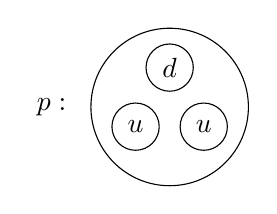
\begin{tikzpicture}
    \node at (0,0) {$p:$};
    \draw (1.500, 0.00) circle (1.0);
    \draw (1.500, 0.50) circle (0.3) node {$d$};
    \draw (1.067,-0.25) circle (0.3) node {$u$};
    \draw (1.933,-0.25) circle (0.3) node {$u$};
  \end{tikzpicture}
  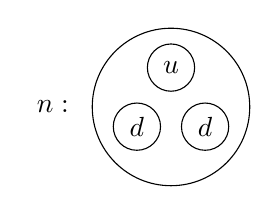
\begin{tikzpicture}
    \node at (0,0) {$n:$};
    \draw (1.500, 0.00) circle (1.0);
    \draw (1.500, 0.50) circle (0.3) node {$u$};
    \draw (1.067,-0.25) circle (0.3) node {$d$};
    \draw (1.933,-0.25) circle (0.3) node {$d$};
  \end{tikzpicture}
  \\
  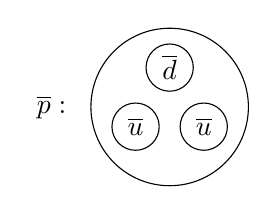
\begin{tikzpicture}
    \node at (0,0) {$\bar{p}:$};
    \draw (1.500, 0.00) circle (1.0);
    \draw (1.500, 0.50) circle (0.3) node {$\bar{d}$};
    \draw (1.067,-0.25) circle (0.3) node {$\bar{u}$};
    \draw (1.933,-0.25) circle (0.3) node {$\bar{u}$};
  \end{tikzpicture}
  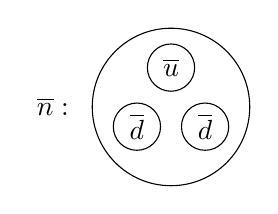
\begin{tikzpicture}
    \node at (0,0) {$\bar{n}:$};
    \draw (1.500, 0.00) circle (1.0);
    \draw (1.500, 0.50) circle (0.3) node {$\bar{u}$};
    \draw (1.067,-0.25) circle (0.3) node {$\bar{d}$};
    \draw (1.933,-0.25) circle (0.3) node {$\bar{d}$};
  \end{tikzpicture}
  \caption{Protons and Neutrons as Quarks}
\end{figure}

\subsection{Beta Decay Again}
We should revisit $\beta$ decay in terms of the constituent quarks of protons and neutrons. We instead see the process as:
\begin{figure}[H]
  \centering
  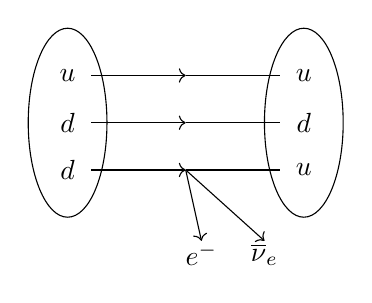
\begin{tikzpicture}
    \draw (0,0) ellipse (0.5 and 1.2);
    \node at (0, 0.6) {$u$};
    \node at (0, 0.0) {$d$};
    \node at (0,-0.6) {$d$};
    \draw (3,0) ellipse (0.5 and 1.2);
    \node at (3, 0.6) {$u$};
    \node at (3, 0.0) {$d$};
    \node at (3,-0.6) {$u$};
    \draw[->] (0.3, 0.6) to (1.5, 0.6);
    \draw[-]  (1.5, 0.6) to (2.7, 0.6);
    \draw[->] (0.3, 0.0) to (1.5, 0.0);
    \draw[-]  (1.5, 0.0) to (2.7, 0.0);
    \draw[->] (0.3,-0.6) to (1.5,-0.6);
    \draw[-]  (1.5,-0.6) to (2.7,-0.6);
    \draw[->] (1.5,-0.6) to (1.7,-1.5) node [yshift=-0.5em] {$e^-$};
    \draw[->] (1.5,-0.6) to (2.5,-1.5) node [yshift=-0.5em] {$\bar{\nu}_e$};
  \end{tikzpicture}
  \caption{$\beta$ decay in terms of quarks}
  \label{fig:beta}
\end{figure}
Thus we can describe the Fermi weak interaction in terms of quarks:
\begin{figure}[H]
  \centering
  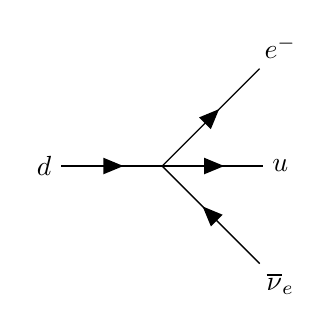
\begin{tikzpicture}
    \begin{feynhand}
      \vertex (a) at (0,0) {$d$};
      \vertex (i) at (1.5,0);
      \vertex (b) at (3,0) {$u$};
      \vertex (e) at (3,1.5) {$e^-$};
      \vertex (n) at (3,-1.5) {$\bar{\nu}_e$};
      \propag[fer] (a) to (i);
      \propag[fer] (i) to (b);
      \propag[fer] (i) to (e);
      \propag[antfer] (i) to (n);
    \end{feynhand}
  \end{tikzpicture}
  \caption{``Four-Fermion'' Fermi Interaction}
  \label{fig:fermi}
\end{figure}

Thus so far, our ``Standard Model'' looks just like:
\begin{gather*}
  \pmqty{u\\d}\\
  \pmqty{\nu_e\\e}
\end{gather*}

However, there is still more to come!


% -*- TeX-master: "master.tex" -*-
\section{Relativity}
Consider two \emph{inertial} frames $S$ and $S'$ with coordinates denoted as $(t,x,y,z)$ and $(t',x',y',z')$ respectively, and coordinated aligned. If $S'$ moves relative to $S$ in the $+x$ direction, with velocity $v$, the coordinates are related in Newtonian mechanics by a Galilean Transformation:
\begin{definition}[Galilean Relativity]
  Galilean Relativity is defined by the transformation from $S$ to a moving frame $S'$. The key assumption is that \emph{time} is the same in every reference frame:
  \begin{align*}
    t=t'
  \end{align*}
  So if $S'$ is moving relative to $S$ in the $+x$ direction with velocity $v$, we have:
  \begin{align*}
    t'=t\quad x'=x-vt\quad y'=y\quad z'=z
  \end{align*}
  Which is called a \emph{Galilean Transformation}
\end{definition}

\emph{Special Relativity} instead assumes the \underline{speed of light} $c$ is the same in every reference frame.

In order to measure the speed of light, it has to travel over some distance in some time, $\therefore$ define an event:
\begin{definition}[Event]
  An event is defined by a physical occurance (light emission for example). It can be defined to occur at the origin of $S$ and $S'$, A second event at $(t,x,y,z)$ or $(t',x',y',z')$ occurs at a position denoted by the coordinates used in a given inertial frame, $S$ or $S'$
\end{definition}

Spacetime then is the collection of our events, the set of which forms a geometry.

Our assumption that $c(t,x,y,z)=c(t',x',y',z')$ implies that, if we use our two events above:
\begin{gather*}
  c=\frac{\sqrt{x^2+y^2+z^2}}{t}=\frac{\sqrt{(x')^2+(y')^2+(z')^2}}{t'}
\end{gather*}
We can then get a quantity that should be equal in all reference frames:
\begin{align*}
  c^2t^2-(x^2+y^2+z^2)=c^2(t')^2-((x')^2+(y')^2+(z')^2)=0
\end{align*}
We can use this quantity to define a sense of distance in spacetime:
\begin{definition}[Spacetime Separation]
  The distance in spacetime from the origin is defined by $\Delta s$:
  \begin{gather*}
    (\Delta s)^2\equiv c^2t^2-(x^2+y^2+z^2)
  \end{gather*}
  An equivalent assumption for special relativity is that the spacetime distance $\Delta s$ is the same in all inertial frames, i.e.\ it is invariant; invariants are \emph{very} useful quantities.
\end{definition}

\subsection{Light Cone}
Earlier we showed that $\Delta s$ for light is $0$. For a general particle, its velocity is always less than $c$, so in the equation for $\Delta s$, the $t$ term dominates, giving $(\Delta s)^2>0$. Note that if $(\Delta s)^2<0$, even light cannot get there. We then define the three regimes of separation:
\begin{table}[H]
  \centering
  \begin{tabular}{ccc}
    $(\Delta s)^2$ & Name & Note \\\hline
    $>0$ & Time-like & Ordinary Masses \\
    $=0$ & Light-like & Particles that travel at $c$ \\
    $<0$ & Space-like & ``Tachyonic'' matter with $v>c$
  \end{tabular}
  \caption{Spacetime Separation Categories}
\end{table}
This then gives the sense that $(\Delta s)^2=0$ forms a surface in 4-space, we call it the light cone:
\begin{figure}[H]
  \centering
  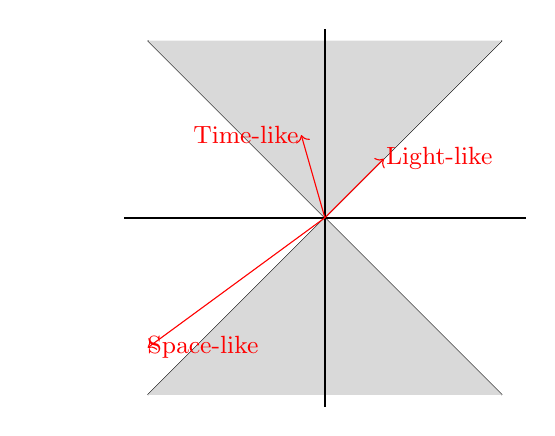
\begin{tikzpicture}[scale=1.5]
    \def\b{0.2} % semi-minor axis
    \pgfmathsetmacro{\h}{(1 + sqrt(1 + 4*\b^2)) / 2}
    \pgfmathsetmacro{\a}{sqrt(\h)}
    \draw (-1.5, -1.5) -- (1.5,  1.5);
    \draw (-1.5,  1.5) -- (1.5, -1.5);
    \fill[gray!30] (0,0) -- (1.5,1.5) -- (-1.5,1.5);
    \fill[gray!30] (0,0) -- (-1.5,-1.5) -- (1.5,-1.5);
    % \draw (0,  \h) ellipse [x radius = \a, y radius = \b];
    % \draw (0, -\h) ellipse [x radius = \a, y radius = \b];
    \draw [thick] (0,-1.6) -- (0,1.6);
    \draw [thick] (-1.7,0) -- (1.7,0);
    \draw [->, red] (0,0) -- (0.5,0.5) node {\hspace{4em}\small Light-like};
    \draw [->, red] (0,0) -- (-0.2,0.7) node {\hspace{-4em}\small Time-like};
    \draw [->, red] (0,0) -- (-1.5,-1.1) node {\hspace{4em}\small Space-like};
  \end{tikzpicture}
  \caption{The Light Cone}
\end{figure}
The gray shaded area is the accessible region of spacetime by light, the lightcone.

\subsection{Time Dilation}



% -*- TeX-master: "master.tex" -*-
\section{Symmetry}
The study of symmetry has been a central theme in the study of physics. In 1917 Emmy Noether proved that (for a specific type of field-complex, 4-dimensional) a symmetry of the Hamiltonian implied the existence of a conserved quantity

You have studied the correspondence of symmetries and conserved quantities in classical and quantum mechanics:
\begin{itemize}
\item Time translation invariance $\iff$ Energy conservation
\item Space translation invariance $\iff$ Momentum conservation
\item Rotational invariance $\iff$ Angular momentum conservation
\end{itemize}

The construction of the Standard Model (and much of theoretical thought) has been largely the identification of the symmetries associated with observed conserved quantities.

\begin{aside}
  Not all conserved quantities must come from symmetries, e.g. solitons and other topological properties etc.
\end{aside}

A conserved quantity is one that is unchanged by a transformation, e.g. a Lorentz scalar under a Lorentz transformation.

The set of possible transformations of a given type have the properties of a \underline{group}. Hence, we study groups and algebras

\subsection{Group Theory}
Reminder of group definitions
\begin{enumerate}
\item Clousure: if $A\in G$, $B\in G$, then $AB\in G$
\item $\exists$ an identity: $I\in G$
\item Every element has an inverse: $A\in G$, $AA^{-1}=A^{-1}A=I$ with $A^{-1}\in G$
\item Associativity: $(AB)C=A(BC)$
\end{enumerate}

\subsubsection{Rotation Group}
Consider rotation by angle $\theta$ about the $z$-axis:
\begin{align*}
  \pmqty{x'\\y'\\z'}=
  \underbrace{\pmqty{\cos\theta & \sin\theta&\\
      -\sin\theta&\cos\theta&\\&&1}}_{R_z(\theta)}
  \pmqty{x\\y\\z}
\end{align*}
Similarly:
\begin{align*}
  R_x(\theta)=
  \pmqty{1\\&\cos\theta&\sin\theta\\&-\sin\theta&\cos\theta}
  \qquad
  R_y(\theta)=
  \pmqty{\cos\theta&&\sin\theta\\&1&\\-\sin\theta&&\cos\theta}
\end{align*}
Two successive rotations is also a rotation (closure). Can you quickly show the other group requirements?

Rotations leave the length of a vector invariant:
\begin{TODO}
  Show above
\end{TODO}

So rotations form a three-dimensional orthogonal group. In addition:
\begin{align*}
  \det{R}=\cos^2\theta+\sin^2\theta=1
\end{align*}
So the rotation group is $SO(3)$, S for special, O for orthogonal.

Recal the Lorentz group is $SO(3,1)$. Rotations are a \underline{subgroup} of the Lorentz Group:
\begin{align*}
  \Lambda^\mu_\nu=\pmqty{\text{Boosts}&\\&3\times3\text{ Rotations}}
\end{align*}
So the Lorentz group $=$ Boosts + Rotations

\subsubsection{Spin}
Consider a particle of mass $m$ at rest. Its four-momentum is:
\begin{align*}
  p^\mu=\pmqty{m\\0\\0\\0}
\end{align*}
Certainly the particle's four-momentum is invariant under rotations. The spin of the particle tells you how the wavefunction of the particle transforms  under the rotation group:
\begin{itemize}
\item Spin 0: $R=\bm{1}$ Trivial
\item Spin $\frac12$: $R_i=\exp{i\frac12\theta_i\sigma_i}$ where $\sigma_i$ are the Pauli matrices $(2\times2)$
\item Spin 1: $R=3\times3$ Rotation matrices (see above)
\item Spin $\frac32$: $R=4\times4$ matrices
\item Spin $j$: $R=(2j+1)\times(2j+1)$ matrices
\end{itemize}
So the spin of a particle is related to its \underline{representation} of the rotation group

Formally, a representation is a homomorphic mapping of a group onto the matrices $(GL_n)$ of rank $n$.

The symmetry associated with rotations is continuous. Hence, rather than work directly with the rotation matrices, we may work with the significantly simpler infinitesimal roations:

Let $R(\theta)=\exp{i\theta_iT_i}\equiv e^{i\theta_iT_i}$, where $T_i$ are matrices, $i=x,y,z$, and $\exp$ of a matrix is just the shorthand for:
\begin{align*}
  \exp{M}=e^M\equiv\sum_{i=0}^\infty\frac{M^n}{n!}
\end{align*}
We know that $R^TR\equiv\bm{1}$, so that $\exp{i\theta_iT_i}^T\exp{i\theta_iT_i}=\bm{1}$. Consider $\theta_i$ to be infinitesimal and expand:
\begin{align*}
  (\bm{1}+i\theta_iT_i^T+\cdots)
  (\bm{1}+i\theta_iT_i^T+\cdots)&=\bm{1}\\
  \implies \theta_i\qty[T_i^T+T_i]&=0
\end{align*}
Thus we arrive at $T_i^T=-T_i$, that is, $T_i$ are \underline{antisymmetric matrices}.

Consider: $R_x(\theta)$ with $\theta\ll 1$:
\begin{align*}
  R_x(\theta\ll1)&=\pmqty{1\\&1&-\theta\\&\theta&1}\\
  &=\bm{1}+\theta\pmqty{0&0&0\\0&0&-1\\0&1&0}
\end{align*}
From above, we can then identify $iT_x$ as this second matrix. Repeating the above process for $R_y,R_z$, we obtain a full set of generators of $SO(3)$:
\begin{align*}
  iT_x=\pmqty{0&0&0\\0&0&-1\\0&1&0}\quad
  iT_y=\pmqty{0&0&-1\\0&0&0\\1&0&0}\quad
  iT_z=\pmqty{0&-1&0\\1&0&0\\0&0&0}
\end{align*}



% -*- TeX-master: "master.tex" -*-
\newcommand{\sla}[1]{\slashed{#1}}
\newcommand{\slap}{\slashed{p}}
\section{Dirac Equation}
Historically, the relativistic Dirac Equation grew out of an attempt to fix the relativistic generalizations of the Schrodinger equation, known as the Klein-Gordon Equation, when applied to the electron (a fermion). A pedagogical derivation of the Dirac Equation typically starts with a massive electron, identifies its equations of motion as a subset of solutions to the Klein-Gordon equation, and then proceeds to modify the equations until they satisfy important properties, like positive-definiteness, and invariance under spatial rotation, etc. You are left with a Dirac Equation which is applied to new objects, called spinors, that can be seen to describe both particles and antiparticles at the same time. This semi-historical approach is taken by most texts (including Griffiths, Halzen\& Martin, etc.)

Here we will take a more modern perspective. In the Standard Model (and beyond), the fields begin by describing \underline{massless} particles and antiparticles; where mass arises from the interactions with other particles. Hence, we will begin from the more general case of examining relativistic states --- representations of the Lorentz group --- and see how they combine to yield the Dirac Equation.

\subsection{Lorentz Group}
Recall the form of $\Lambda^\mu_\nu$:
\begin{align*}
  \Lambda^\mu_\nu&=\pmqty{\gamma&&&\beta\gamma\\&1\\&&1\\\beta\gamma&&&\gamma}
  \underset{\beta\to\veps_z\ll 1}{\to}\bm{1}+\veps_z\pmqty{&&&1\\ \\ \\ 1}\\
  &\equiv\exp{i\veps_z K_z}=\bm{1}+i\veps_z K_z\\
  \implies iK_z&=\pmqty{&&&1\\ \\ \\1}
\end{align*}
So as we did before, we can construct generators of Lorentz boosts:
\begin{align*}
  K_x=-i\pmqty{0&1&0&0\\1&0&0&0\\0&0&0&0\\0&0&0&0}\quad
  K_y=-i\pmqty{0&0&1&0\\0&0&0&0\\1&0&0&0\\0&0&0&0}\quad
  K_z=-i\pmqty{0&0&0&1\\0&0&0&0\\0&0&0&0\\1&0&0&0}
\end{align*}
Note that $K^\dag_i=-K_i$, they are anti-Hermitian

\begin{aside}
  The Structure of the Lorentz Group is 3 Boosts and 3 Rotations, the group is $SO(3,1)$. Rotations are a $SO(3)$ subgroup of the Lorentz group, but boosts are NOT:\@
  \begin{align*}
    \Lambda^\mu_\nu=
    \begin{tabular}{c|ccccc}
        & b  & o  & o  & s  & t \\ \hline
      b & ro &    &    &    &   \\
      o &    & ta &    &    &   \\
      o &    &    & ti &    &   \\
      s &    &    &    & on &   \\
      t &    &    &    &    & s
    \end{tabular}
  \end{align*}
  A subgroup would correspond to block matrices in the greater matrix.
\end{aside}
The Lie Algebras of Relativity involve these boost and rotation matrices:
\begin{align*}
  \comm{K_i}{K_j}&=-i\veps_{ijk}J_k\\
  \comm{J_i}{J_j}&= i\veps_{ijk}J_k\\
  \comm{J_i}{K_j}&= i\veps_{ijk}K_k
\end{align*}
To study the representations of the Lorentz group, it is useful to form a new basis of generators:
\begin{align*}
  A_i&=\frac12(J_i+iK_i)\\
  B_i&=\frac12(J_i-iK_i)\\
\end{align*}
Notice that $A_i^\dag=A_i$ and $B_i^\dag=B_i$.

It can then be shown the new Lie Algebra is:
\begin{align*}
  \comm{A_i}{A_j}&=i\veps_{ijk}A_k\\
  \comm{B_i}{B_j}&=i\veps_{ijk}B_k\\
  \comm{A_i}{B_j}&=0
\end{align*}
\begin{proof}
  \begin{align*}
    \comm{A_i}{A_j}&=\frac14\qty(
    \comm{J_i}{J_j}+i\comm{K_i}{J_j}+i\comm{J_i}{K_j}-\comm{K_i}{K_j})\\
    &=\frac14\qty(
    i\veps_{ijk}J_k+i(-i)\veps_{ijk}K_k+ii\veps_{ijk}K_k+i\veps_{ijk}J_k)\\
    &=\frac12\qty(i\veps_{ijk}(J_k+iK_k))=i\veps_{ijk}A_k
  \end{align*}
\end{proof}
This means $A_i$ and $B_i$ each satisfy the Lie algebra of $SU(2)$ independently! This means:
\begin{align*}
  SO(3,1)\equiv SU{(2)}_A\otimes SU{(2)}_B
\end{align*}

\begin{remark}
  \underline{\bf WARNING}, These $SU(2)$ have nothing to do with any other $SU(2)$ we've studied, and neither one corresponds to pure rotations. 
\end{remark}

The representations of the Lorentz group can now be expressed by the representations of $(A,B)$.

\subsubsection{(2,0) Representation}
Simplest reoresentation: $(A,B)=(2,0)$, also called $\qty(\frac12,0)$. This corresponds to $A_i=\frac12\sigma_i$ and $B_i=0$, the $A$'s have the algebra of spin-$\frac12$, and the $B$'s have the algebra of spin-0.

So the (2,0) representation describes a \underline{massless}, spin-$\frac12$ ferion of helicity $+\frac12$, this is called a Weyl (or chiral) fermion.

Let $p^\mu=(E,0,0,E)$. Then $\vu{p}=(0,0,1)$, and Helicity $h=\frac12\bm{\sigma}\vdot\vu{p}$.

Lets find the two-component state $\psi$ acted upon by $h$:
\begin{align*}
  h\psi&=\frac12(\bm{\sigma}\vdot\vu{p})\psi=+\frac12\psi\\
  &=\frac12\sigma_z\psi=+\frac12\psi
\end{align*}
The first line tells us that $\psi$ has $h=+\frac12$, the second tells us the specific form of $\psi$ in terms of a vector since we know the form of $\sigma_z$:
\begin{align*}
  \psi=\pmqty{1\\0}
\end{align*}
It is tempting to then say $\psi=\pmqty{0\\1}$ is a particle with $h=-\frac12$, but it \underline{does not}! It still have $h=\frac12$:
\begin{proof}
  Rotate about the $x$-axis by $\theta=\pi$:
  \begin{align*}
    \psi'=e^{i\sigma/2\vdot\theta}\psi=e^{i\pi\sigma_x/2}\psi
  \end{align*}
  Use Euler's Formula:
  \begin{align*}
    e^{i/2\bm{\sigma}\vdot\theta}=\bm{1}\cos(\frac\theta2)+
    i(\bm{\sigma}\vdot\hat{\bm{\theta}})\sin(\frac\theta2)
  \end{align*}
  This means that:
  \begin{align*}
    \psi'=i\sigma_x\psi=i\pmqty{&1\\1}\pmqty{1\\0}=i\pmqty{0\\1}
  \end{align*}
  To find the Helicty, we need to rotate $\vu{p}\to\vu{p}'$:
  \begin{align*}
    {(p')}^\mu=\pmqty{
      1&0&0&0\\
      0&1&0&0\\
      0&0&\cos\theta&\sin\theta\\
      0&0&-\cos\theta&\cos\theta
    }
    \pmqty{E\\0\\0\\E}=\pmqty{E\\0\\E\sin\theta\\E\cos\theta}
  \end{align*}
  Which reduced to $(E,0,0,-E)$ for $\theta=\pi$, so $\vu{p}'=(0,0,-1)$. So the rotated helicity operator on the rotated state gives:
  \begin{align*}
    \frac12(\bm{\sigma}\vdot\vu{p}')\psi'=\frac12(-\sigma_z)\psi'
    =-\frac12\pmqty{1\\&-1}\pmqty{0\\i}=\frac12\pmqty{0\\i}=+\frac12\psi'
  \end{align*}
  $\therefore h=+\frac12$ in primed frame!
\end{proof}

The helicity of a massless particle is also boost invariant. To see this let's revisit boosts to establish notation:
\begin{align*}
  \Lambda^\mu_\nu&=\pmqty{\gamma&&&\beta\gamma\\&1\\&&1\\\beta\gamma&&&\gamma}
  =\pmqty{\cosh\eta&&&\sinh\eta\\&1\\&&1\\\sinh\eta&&&\cosh\eta}
\end{align*}
Where $\eta$ is the ``rapidity'' --- an analog of $\theta$ for rotations.

\begin{gather*}
  \beta=\tanh\eta=\frac{e^\eta-e^{-\eta}}{e^\eta+e^{-\eta}}\\
  -\infty<\eta<\infty
\end{gather*}

Go back to (2,0), and this time, instead of rotating along $x$, boost in $x$ by $\eta$:
\begin{align*}
  \psi'=e^{1/2\bm{\sigma}\vdot\bm{\eta}}\psi=e^{1/2\sigma_x\eta}\psi
\end{align*}
Use the fact that $\cosh$ and $\sinh$ are the even/odd decompositions of the exponential:
\begin{align*}
  \psi'&=\qty(\cosh(\frac\eta2)+\sigma_x\sinh(\frac\eta2))\psi\\
  &=\pmqty{\cosh(\eta/2)\\\sinh(\eta/2)}
\end{align*}
The boosted momentum is:
\begin{align*}
  {(p')}^\mu=\pmqty{\cosh\eta&\sinh\eta\\\sinh\eta&\cosh\eta\\&&1\\&&&1}
  \pmqty{E\\0\\0\\E}=\pmqty{E\cosh\eta\\E\sinh\eta\\0\\E}
\end{align*}
So $\vu{p}'=(\sinh\eta,0,1)/\sqrt{1+\sinh^2\eta}=(\tanh\eta,0,\sech\eta)$

And the helicity is:
\begin{align*}
  h=\frac12(\bm{\sigma}\vdot\vu{p}')\psi'&=\frac12
  \qty(\sigma_x\tanh\eta+\sigma_z\sech\eta)\pmqty{\cosh\eta/2\\\sinh\eta/2}\\
  &=\frac12\qty(\tanh\eta\pmqty{\sinh\eta/2\\\cosh\eta/2}
  +\sech\eta\pmqty{\cosh\eta/2\\-\sinh\eta/2})
\end{align*}
You can use sum and difference of the argument to simplify this to:
\begin{align*}
  h&=\frac12\sech\eta\pmqty{
    \sinh\eta\sinh\eta/2+\cosh\eta/2\\
    \sinh\eta\cosh\eta/2-\sinh\eta/2
  }\\
  &=\frac12\sech\eta\pmqty{
    \cosh\eta\cosh\eta/2\\
    \cosh\eta\sinh\eta/2
  }
  =\frac12\pmqty{
    \cosh\eta/2\\
    \sinh\eta/2
  }
\end{align*}
Hence, the helicity is still $\frac12$! This means the $(2,0)$ representation of the Lorentz group describes a massless fermion with $h=+\frac12$. We call this a \underline{right-handed} spinor. It satisfies:
\begin{align*}
  (\bm{\sigma}\vdot\vu{p})\psi=\psi
\end{align*}

Now, $p^\mu=(E,E\vu{p})$, so we can write the above equation as:
\begin{align*}
  (p^\mu\sigma_\mu)\psi=0
\end{align*}
Where $\sigma^0=\bm{1}$, $\sigma^i=$Pauli Matrices. Multiply on the left with $\psi^\dag$:
\begin{align*}
  \implies\psi^\dag p^\mu\sigma_\mu\psi=p^\mu(\psi^\dag\sigma_\mu\psi)=0
\end{align*}
This implies that the parenthetical term $\psi^\dag\sigma^\mu\psi$ transforms as a massless four-vector, $v^\mu=\psi^\dag\sigma^\mu\psi$. Since $v^\mu$ contracted with $p^\mu$ is 0 and $p^\mu p_\mu=0$ for a massless particle, we know $v^\mu$ must be proportional to $p^\mu$: $v^\mu=\alpha v^\mu$. This transforms our $2\otimes2$ representation into a single 4-vector representation, $2\otimes2=4$

\subsubsection{(0,2) Representation}
The $(0,2)$ or $\qty(0,\frac12)$ representation corresponds to a massless \underline{left-handed} state, $h=-\frac12$. This is given by:
\begin{align*}
  J_i=\frac12\sigma_i\qquad iK_i=-\frac12\sigma_i
\end{align*}
Let $p^\mu=(E,0,0,E)$, $\psi=(0,1)$, we could then show that $h\psi=-\frac12\psi$, same as before.

\subsubsection{(2,0) $\oplus$ (0,2) Representation}
The helicity of a massless particle is a Lorentz-invariant concept, as we've seen. Of course, this is not true of a massive particle. For example, consider a particle with $h=+\frac12$, this means its spin and momentum are in the same direction, lets say in $+z$. By boosting in the $-z$ direction, the momentum can be flipped, but the helicity will not be, resulting in a helicity of $-\frac12$. Contrast this with a massless particle, no such boost exists.

To describe massive particles then, we will need both right and left handed spinors.

If we add the two massless four-vectors with equaal energy, but opposite momentum, we get a massive particle at rest:
\begin{align*}
  p_1^\mu&=(E,0,0,E)\\
  p_2^\mu&=(E,0,0,2E)\\
  {(p_1+p_2)}^\mu&=(2E,0,0,0)
\end{align*}
So the mass $m=2E$

Let's add these states such that one is left-handed, one right-handed, but both have $s_z=+\frac12$:
\begin{align*}
  \psi_R\oplus\psi_L=\pmqty{1\\0}\oplus\pmqty{1\\0}
\end{align*}
Note the helicity of $\psi_L$ is $\frac12(\bm{\sigma}\vdot\vu{p})\psi_L=-\frac12\sigma_z=-\frac12\psi$. We then have $u_+$:
\begin{align*}
  U_+=\pmqty{\psi_R\\\psi_L}=\pmqty{1\\0\\1\\0}
\end{align*}
This is a \underline{Dirac spinor}. It corresponds to a massive particle at \underline{rest} with $s_z=+\frac12$:
\begin{align*}
  s_z u_+=\frac12\pmqty{\sigma_z\\&\sigma_z}u_+=+\frac12 u_+
\end{align*}
To obtain a right handed spinor of arbitrary momentum, boost along the $z$-axis, then rotate into the desired direction:
\begin{align*}
  \text{Rotation:}&\quad u_+'=
  \pmqty{e^{i/2\sigma\vdot\theta}\\&e^{i/2\sigma\vdot\theta}}
  \pmqty{\psi_R\\\psi_L}\\
  \text{Boost:}&\quad u_+'=
  \pmqty{e^{1/2\sigma\vdot\eta}\\&e^{-1/2\sigma\vdot\eta}}
  \pmqty{\psi_R\\\psi_L}
\end{align*}
First boost along $z$, with $\eta=(0,0,\eta)$:
\begin{align*}
  u_+=\pmqty{e^{1/2\sigma_z\eta}\\&e^{-1/2\sigma_z\eta}}\pmqty{1\\0\\1\\0}
  =\pmqty{e^{\eta/2}\\0\\e^{-\eta/2}\\0}
\end{align*}
Recall:
\begin{align*}
  e^\eta&={\qty(\frac{1+\beta}{1-\beta})}^{\frac12}\\
  \beta&=\frac{p}{E}\\
  e^\eta&={\qty(\frac{E+p}{E-p})}^{\frac12}
\end{align*}
So we get $u_+'$ as:
\begin{align*}
   u_+'={\pmqty{((E+p)/(E-p))^{1/4}\\0\\{((E-p)/(E+p))}^{1/4}\\0}}
\end{align*}
It is conventional (and sensible) to normalize $u_\pm^\dag u_\pm=2E$:
\begin{align*}
  u_+'=\sqrt{m}\pmqty{{((E+p)/(E-p))}^{1/4}\\0\\{((E-p)/(E+p))}^{1/4}\\0}
  =\pmqty{{(E+p)}^{1/2}\\0\\{(E-p)}^{1/2}\\0}
\end{align*}
Now rotate about the $y$-axis by angle $\theta$ using
$e^{i/2\sigma_y\theta}=\bm{1}\cos(\theta/2)+i\sigma_y\sin(\theta/2)$:
\begin{align*}
  u_{+}&=\pmqty{
    {(E+p)}^{1/2}\pmqty{\cos\theta/2\\-\sin\theta/2}
    {(E-p)}^{1/2}\pmqty{\cos\theta/2\\-\sin\theta/2}
  }\\
  u_{-}&=\pmqty{
    {(E-p)}^{1/2}\pmqty{\sin\theta/2\\\cos\theta/2}
    {(E-p)}^{1/2}\pmqty{\sin\theta/2\\\cos\theta/2}
  }
\end{align*}
Note you can find $u_-$ by starting from the $(0,1,0,1)$ state in the rest frame.

Note in the $m=0$ limit, when $E\to p$, and if $\theta=0$:
\begin{align*}
  u_+=\sqrt{2E}\pmqty{1\\0\\0\\0}\qquad
  u_-=\sqrt{2E}\pmqty{0\\0\\0\\1}
\end{align*}
Which recovers our normalized massless representations. The massless spinors satisfy certain constraints, like (2,0) has $(p^\mu\sigma_\mu)\psi_R=0$:
\begin{align*}
  \implies\qty[p^0\pmqty{\bm{1}\\&\bm{1}}-p^i\pmqty{\sigma^i\\&-\sigma^-}]
  \pmqty{\psi_R\\\psi_L}=0
\end{align*}
Now consider a massive spinor. Take $u_+$ with $p^\mu=(E,0,0,p)$:
\begin{align*}
  \qty(p^0\bm{1}-p\sigma_z)\psi_R=
  (E-p)\pmqty{{(E+p)}^{1/2}}=m\pmqty{{(E-p)}^{1/2}}
  =m\psi_L
\end{align*}
Similarly:
\begin{align*}
  \qty(p^0\bm{1}-p\sigma_z)\psi_L
  =(E+p)\pmqty{{(E-p)}^{1/2}}=m\pmqty{{(E+p)}^{1/2}}
  =m\psi_R
\end{align*}
Thus:
\begin{align*}
  \qty[p^0\pmqty{\bm{1}\\&\bm{1}}-p^i\pmqty{\sigma^i\\&-\sigma^-}]
  \pmqty{\psi_R\\\psi_L}=m\pmqty{\psi_L\\\psi_R}
\end{align*}
Notice that $L/R$ swap! We can fix this by multiplying by the matrix $\gamma^0$:
\begin{align*}
  \gamma^0=\pmqty{&\bm{1}\\\bm{1}}
\end{align*}
This results in:
\begin{align*}
  \qty[p^0\pmqty{&\bm{1}\\\bm{1}}-p^i\pmqty{&-\sigma^i\\\sigma^-}]
  \pmqty{\psi_R\\\psi_L}=m\pmqty{\psi_R\\\psi_L}
\end{align*}
Define $\gamma^i$ and $\gamma^\mu$:
\begin{align*}
  \gamma^i&\equiv\pmqty{&-\sigma^i\\\sigma^-}\\
  \implies\gamma^\mu&=(\gamma^0,\gamma^i)
\end{align*}
The equation then becomes:
\begin{align*}
  p^\mu\gamma_\mu u_+=m u_+
\end{align*}
We Then define ``slash'' notation:
\begin{definition}[Slash Notation]
  We can simplify this stuff with the gamma matrices using slash notation:
  \begin{align*}
    a^\mu\gamma_\mu\equiv \sla{a}\implies
    \sla{p}u_+=mu_+
  \end{align*}
\end{definition}
We could repeat this exercise for $u_-$ and find the same result, we then have the \underline{Dirac equation}:
\begin{align*}
  \sla{p}u=mu
\end{align*}
This is written in momentum space. Amazingly, we've shown that this is just a constraint equation that must be satisfied by a massive spinor!

\begin{aside}
  Note the $\gamma$ matrices:
  \begin{align*}
    \gamma^0=\pmqty{&\bm1\\\bm{1}}\qquad
    \gamma^i=\pmqty{&-\sigma^i\\\sigma^i}
  \end{align*}
  Recall the Pauli matrices anticommute: $\acomm{\sigma^i}{\sigma^j}=2\delta^{ij}$. One can show a similar relation with these matrices:
  \begin{align*}
    \acomm{\gamma^\mu}{\gamma^\nu}=2g^{\mu\nu}
  \end{align*}
  This defines a \underline{Clifford Algebra}
\end{aside}

Since we built the ``Dirac'' $\gamma$ matrices and spinors from explicit chiral (handed) representations (2,0) and (0,2), this for mof the $\gamma$ matrices and spinors is called the chiral representation. There are other representations, notably the \underline{Dirac} representation (originally found by Dirac) that appears in most textbooks.

You can obtain the Dirac representation from the chiral one by a unitary transformation:
\begin{align*}
  \gamma^\mu_{Dirac}&=U\gamma^\mu U^\dag\\
  U&=\frac1{\sqrt{2}}\pmqty{\bm{1}&\bm{1}\\\bm{1}&-\bm{1}}
\end{align*}
We can still use the $\gamma$ matrices for massless spinors. Define $\gamma_5$:
\begin{align*}
  \gamma_5&=\pmqty{\bm{1}\\&-\bm{1}}\\
  \frac12\qty(\bm{1}+\gamma_5)&=\pmqty{\bm{1}\\&0}\\
  \frac12\qty(\bm{1}-\gamma_5)&=\pmqty{0\\&\bm{1}}
\end{align*}
Use these to project out $\psi_R$ and $\psi_L$. Also note:
\begin{align*}
  \acomm{\gamma^\mu}{\gamma^5}=0
\end{align*}

\begin{aside}
  The $5$ in $\gamma_5$ is not a Lorentz index, just a way to suggectively remind you of Dirac matrices. Also:
  \begin{align*}
    \gamma_5=\gamma^5=\pmqty{\bm{1}\\&-\bm{1}}
  \end{align*}
  Just in case I write one over the other.
\end{aside}

\subsubsection{Antiparticles}
In QFT, the Dirac field is given by:
\begin{align*}
  \psi(x)=\int\frac{\dd[3]{p}}{2E}e^{-ip\vdot x}a u(p)
\end{align*}
Where $a$ is the ``destruction'' or ``annihilation'' operator. We have the following:
\begin{align*}
  \D_\mu\psi&=\int\frac{\dd[3]{p}}{2E}e^{-ip\vdot x}a(-i)p_\mu u(p)\\
  \implies i\sla{\D}\psi&=\int\frac{\dd[3]{p}}{2E}e^{-ip\vdot x}a\sla{p}u(p)\\
  \implies i\sla{\D}\psi&=\int\frac{\dd[3]{p}}{2E}e^{-ip\vdot x}amu(p)\\
  \implies i\sla{\D}\psi&=m\psi
\end{align*}
Quantum field theory also requires antiparticles:
\begin{align*}
  \psi(x)=\int\frac{\dd[3]{p}}{2E}
  \qty[e^{-ip\vdot x}a u(p)+e^{ip\vdot x}b^\dag v(p)]
\end{align*}
Where $b^\dag$ is the ``creation'' operator of the antiparticle.

For this to hold, we must have:
\begin{align*}
  \slap v= -mv
\end{align*}
Where $v$ is an ``antiparticle'' spinor.

We can build $v$ from $(2,0)\otimes(0,2)$. In the rest frame, the unormalized rest frame spinors are:
\begin{align*}
  v_+=\pmqty{1\\0\\-1\\0}\qquad
  v_+=\pmqty{0\\-1\\0\\1}
\end{align*}
Boosting and rotating as before, we get:
\begin{align*}
  v_{+}&=\pmqty{
    {(E+p)}^{1/2}\pmqty{\cos\theta/2\\-\sin\theta/2}
    {(E-p)}^{1/2}\pmqty{-\cos\theta/2\\\sin\theta/2}
  }\\
  v_{-}&=\pmqty{
    {(E-p)}^{1/2}\pmqty{-\sin\theta/2\\-\cos\theta/2}
    {(E+p)}^{1/2}\pmqty{\sin\theta/2\\\cos\theta/2}
  }
\end{align*}
Again $v^\dag v=2E=u^\dag u$.

Consider the product of two spinors:
\begin{align*}
  u^\dag u=\pmqty{\psi_R\\\psi_L}^\dag\pmqty{\psi_R\\\psi_L}
\end{align*}
This is rotation invariant, since $\psi_R$ and $\psi_L$ transform the same way, but it is \underline{not} boost invariant, since the way $\psi_R$ and $\psi_L$ transform differs by a sign in the exponential. Notice however that:
\begin{align*}
  u^\dag\gamma^0u=\pmqty{\psi_R\\\psi_L}^\dag
  \pmqty{&\bm{1}\\\bm{1}}
  \pmqty{\psi_R\\\psi_L}
\end{align*}
Is in fact boost invariant. Thus, we define:
\begin{align*}
  \bar{u}\equiv u^\dag\gamma^0
\end{align*}
Then, $\bar{u}u$ is a Lorentz invariant quantity

Inverting $\gamma_5$ does not affect Lorentz invariance, since it is diagonal. This means that $\bar{u}\gamma_5 u$ is also Lorentz invariant.

Lets re-examine $u^\dag u$ when $u$ is in its rest frame:
\begin{align*}
  u_+=\sqrt{m}\pmqty{1\\0\\0\\0}
\end{align*}
Under a boost in the $z$ direction:
\begin{align*}
  u^\dag_+u_+=2m\implies m\pmqty{1&0&0&0}
  \pmqty{e^\eta\\&e^\eta}\pmqty{1\\0\\0\\0}=m(e^\eta+e^{-\eta})
  =2m\cosh\eta
\end{align*}
So $u^\dag u$ is transforming like the energy component of a massive four-vector: $E'=m\cosh\eta$:
\begin{align*}
  \pmqty{\gamma&&&\beta\gamma\\&1\\&&1\\\beta\gamma&&&\gamma}
  \pmqty{m\\0\\0\\0}=\pmqty{m\cosh\eta\\0\\0\\m\sinh\eta}
\end{align*}
Consider:
\begin{align*}
  \pmqty{\psi_R\\\psi_L}^\dag\pmqty{\sigma^i\\&-\sigma^i}\pmqty{\psi_R\\\psi_L}
\end{align*}
This is a three-vector under rotations and boosts, consider the same spinor as before, boosted in the $z$ direction
\begin{align*}
  &m\pmqty{1\\0\\1\\0}^T
  \pmqty{e^{\sigma_z\eta/2}\\&e^{-\sigma_z\eta/2}}
  \pmqty{\sigma^i\\&-\sigma^i}
  \pmqty{e^{\sigma_z\eta/2}\\&e^{-\sigma_z\eta/2}}
  \pmqty{1\\0\\1\\0}\\
  =&m\pmqty{1\\0\\1\\0}^T
  \pmqty{e^{\eta/2}\\&e^{-\eta/2}}
  \pmqty{\sigma^i\\&-\sigma^i}
  \pmqty{e^{\eta/2}\\&e^{-\eta/2}}
  \pmqty{1\\0\\1\\0}\\
  =&m(\underbrace{e^\eta-e^{-\eta}}_{2\sinh\eta})
  \pmqty{1\\0}^T\sigma^i\pmqty{1\\0}
\end{align*}
Which is exactly how a massive four-vector transforms!

Combine these terms:
\begin{align*}
  u^\dag\qty[\pmqty{\dmat{\bm{1},\bm{1}}},\pmqty{\dmat{\sigma^i,-\sigma^i}}]u
\end{align*}
If we insert an identity in the form of ${(\gamma^0)}^2$ after $u^\dag$, we get:
\begin{align*}
  \bar{u}\gamma^\mu u
\end{align*}
Is a 4-vector, once again inserting $\gamma_5$ also gives a 4-vector:
\begin{align*}
  \bar{u}\gamma^\mu\gamma_5u
\end{align*}
The only other unique product we can form is $\frac{i}2\bar{u}\comm{\gamma^\mu}{\gamma^\nu}u$ --- an antisymmetric tensor.
\begin{table}[H]
  \centering
  \begin{tabular}{ccc}
    $\Gamma$ & Type & Dimension \\\hline
    1 & scalar & 1 \\
    $\gamma_5$ & pseudoscalar & 1 \\
    $\gamma^\mu$ & vector & 4 \\
    $\gamma^\mu\gamma_5$ & vector & 4 \\
    $\frac{i}2\comm{\gamma^\mu}{\gamma^\nu}$ & antisymmetric tensor & 6
  \end{tabular}
  \caption{Summary of objects of the form $\bar{u}\Gamma u$}\label{tab:bilinears}
\end{table}
Combining two dirac spinors we get:
\begin{align*}
  4\otimes4=1\oplus1\oplus4\oplus4\oplus6
\end{align*}

\subsubsection{Parity}
The symmetries of space-time are given by the matrix $\Lambda$, where $\Lambda^T g\Lambda=g$. There is a discrete symmetry given by:
\begin{align*}
  \Lambda=\pmqty{\dmat{1,-1,-1,-1}}
\end{align*}
Which flips the three-momentum of a vector, this operation is called \underline{parity}.

A 3-vector is odd under parity:
\begin{align*}
  P\vb{v}=-\vb{v}
\end{align*}
An axial vector, like $\vb{r\times p}$ is even under parity:
\begin{align*}
  P(\vb{r\times p})=(-\vb{r})\times(-\vb{p})=\vb{r\times p}
\end{align*}
A scalar is even under parity:
\begin{align*}
  P(\vb{r\vdot p})=\vb{r\vdot p}
\end{align*}
A pseudoscalar is odd under parity:
\begin{align*}
  P[\vb{q}\vdot(\vb{r\times p})]={(-1)}^3\vb{q}\vdot\vb{r\times p}
\end{align*}
Spin (angular momentum) does not flip under parity (it is an axial vector), but $\vb{p}$ does, so helicity flips under parity.

So, under parity, $\psi_R$ swaps with $\psi_L$, along with the momentum flipping. So this means $u$ is even under Parity:
\begin{align*}
  u_+=\pmqty{{(E+p)}^{1/2}\\0\\{(E-p)}^{1/2}\\0}
  \overset{P}{\rightarrow}\pmqty{{(E+p)}^{1/2}\\0\\{(E-p)}^{1/2}\\0}
\end{align*}
While $v$ is odd:
\begin{align*}
  v_+=\pmqty{{(E+p)}^{1/2}\\0\\-{(E-p)}^{1/2}\\0}
  \overset{P}{\rightarrow}\pmqty{-{(E+p)}^{1/2}\\0\\{(E-p)}^{1/2}\\0}=-v_+
\end{align*}

% -*- TeX-master: "master.tex" -*-
\section{Quantum Electrodynamics}
In deriving the Dirac equation, we formed Lorentz invariants out of Dirac spinors such as $\bar{\psi}\psi$.

Under the Lorentz group, $\bar{\psi}\psi$ is a scalar, $\bar{\psi}\gamma^\mu\psi$ is a 4-vector, so $\bar{\psi}\sla{\D}\psi$ is also a scalar.

We want a Lagrangian $\L$ invariant under the Lorentz group:
\begin{align*}
  \L=i\bar{\psi}\sla{\D}\psi-m\bar{\psi}\psi
\end{align*}
Equation of motion comes from the Principle of Least Action:
\begin{align*}
  \fdv{\L}{\bar{\psi}}=0\implies i\sla{D}\psi-m\psi=0
\end{align*}
Recall that the other term from the Euler-Lagrange is just $0$ since theres no derivatives of $\bar{\psi}$.

In addition to the Lorentz group, $\L$ is also invariant under the following symmetry:
\begin{align*}
  \psi&\to e^{iQ\theta}\psi\\
  \bar{\psi}&\to \bar{\psi}e^{-iQ\theta}
\end{align*}
Where $Q\in\mathbb{R}$, a $U(1)$ symmetry.

This is a \underline{global} symmetry, $\theta$ is the same over all spacetime. The symmetry group is $U(1)$. QED is introduced by demanding the $U(1)$ symmetry be \underline{local}, where $\theta=\theta(x)$ can change smoothly.

Clearly $m\bar{\psi}\psi$ is invariant:
\begin{align*}
  m\bar{\psi}\psi\to m\bar{\psi}e^{-iQ\theta(x)}e^{iQ\theta(x)}\psi
  =m\bar{\psi}\psi
\end{align*}
The other term:
\begin{align*}
  i\bar{\psi}\sla{\D}\psi\to
  \bar{\psi}e^{-iQ\theta(x)}\sla{\D}(e^{iQ\theta(x)}\psi)
  &=\bar{\psi}e^{-iQ\theta(x)}e^{iQ\theta(x)}\sla{\D}\psi
  +iQ\bar{\psi}\gamma^\mu\psi(\D_\mu\theta)\\
  &=i\bar{\psi}\sla{\D}\psi+i\bar{\psi}(iQ\sla{\D}\theta)\psi
\end{align*}
Is not invariant.

This is remedied by introducing a new field $A^\mu$, into the Lagrangian, and demanding $A^\mu$ transform in just the right way to cancel the offending term. Try the following:
\begin{align*}
  \L=i\bar{\psi}(+ieQ\sla{A})\psi
\end{align*}
Where $\sla{A}=A_\mu\gamma^\mu$, the photon field

The second term in the transformation of $i\bar{\psi}\sla{\D}\psi$ is cancelled if:
\begin{align*}
  A^\mu\to A^\mu-\frac1e\D^\mu\theta(x)
\end{align*}
This local transformation is called a \underline{gauge} transformation, and we say $\L$ is gauge invariant.

The field $A^\mu$ corresponds to the vector potential of the electromagnetic field, and $eQ$ is the electric charge of the fermion.
\begin{itemize}
\item $e$ is called the coupling constant $\alpha=e^2/4\pi\approx 1/137$ is the fine structure constant
\item $Q$ is the charge of particle in units of $e$, $Q=-1$ for electrons, and $Q=+\frac23$ for up quark, etc.
\end{itemize}
The quantum of the EM field is the photon. A mass term in $\L$ would be:
\begin{align*}
  -\frac12M^2A^\mu A_\mu
\end{align*}
But this is \underline{not} gauge invariant. We regard the masslessness of the photon as being a consequence of gauge invariance (although the inverse transformation is also reasonable).

The photon is a massless spin-1 particle and transforms as the $(1,0)\oplus(0,1)$ representation of the Lorentz group. It therefore as helicity $h=\pm1$.

Due to gauge invariance, $A_\mu\to A_\mu-\frac1e\D_\mu\theta$, we can always find a gauge (some $\theta(x)$) where:
\begin{align*}
  \D_\mu A^\mu=0
\end{align*}
This is called the Lorentz gauge, so called because of its manifest Lorentz invariance.

The photon field is:
\begin{align*}
  A^\mu(x)=\int\frac{\dd[3]{p}}{2E}\qty[
  e^{-ip\vdot x}a_\lambda\veps^\mu_\lambda(p)+
  e^{+ip\vdot x}a^\dag_\lambda\veps^{\mu*}_\lambda(p)
  ]
\end{align*}
Where $a,a^\dag$ are the destruction and creation operators for the photon, and $\veps^\mu_\lambda(p)$ is a four-vector which transforms as either the $(1,0)$ rep ($\lambda=+1$), or the $(0,1)$ rep ($\lambda=-1$) of the Lorentz group.

Recall $\psi(x)$:
\begin{align*}
  \psi(x)=\int\frac{\dd[3]{p}}{2E}\qty[
  e^{-ip\vdot x}a_\lambda u_\lambda(p)+
  e^{+ip\vdot x}b^\dag_\lambda v_\lambda(p)
  ]
\end{align*}
The Lorentz gauge condition implies:
\begin{align*}
  p_\mu\veps^\mu_\lambda(p)=0
\end{align*}
This means $\veps^\mu_\lambda$ is the Fourier transform of the photon field, and implies the photon is its own antiparticle.

The ``polarization vectors'' $\veps^\mu_\lambda$ for a photon with momentum $p^\mu=(E,0,0,E)$ are:
\begin{align*}
  \veps^\mu_+&=\frac1{\sqrt{2}}(0,1,i,0)\\
  \veps^\mu_-&=\frac1{\sqrt{2}}(0,1,-i,0)
\end{align*}

\begin{aside}
  Lorentz group (photon not massless) $\lambda=0,\pm1$, for a real photon we would have to remove $\lambda=0$. The radiation gauge, $A^0=0, \grad_i\vdot A^i$, $\lambda=\pm1$ manifestly.
\end{aside}

\subsection{Perturbation Theory}
QED is a weakly-coupled theory -- photons and electrons (or quarks) do not interact very strongly. To zeroth order they do not interact at all. Hence, one can regard interactions as perturbations of this simple picture. The outcome of treating QED perturbatively can be represented pictorially via Feynman diagrams. These ``Feynman rules'' are derived from quantum field theory. In practice, all one needs for simple calculations are the Feynman rules.

Lets draw the Feynman diagram for $e^+e^-\to\mu^+\mu^-$ then work out the details:
\begin{figure}[H]
  \centering
  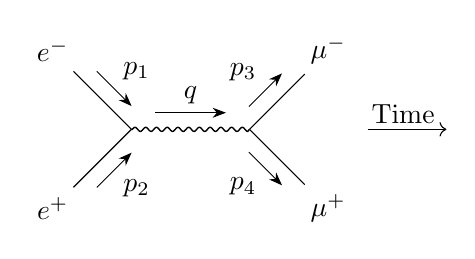
\begin{tikzpicture}
    \begin{feynhand}
      \vertex (a) at (0,0);
      \vertex (e1) at (-1, 1) {$e^-$};
      \vertex (e2) at (-1,-1) {$e^+$};
      \vertex (m1) at (2.5, 1) {$\mu^-$};
      \vertex (m2) at (2.5,-1) {$\mu^+$};
      \vertex (b) at (1.5,0);
      \propag[mom=\(p_1\)] (e1) to (a);
      \propag[mom'=\(p_2\)] (e2) to (a);
      \propag[mom=\(p_3\)] (b) to (m1);
      \propag[mom'=\(p_4\)] (b) to (m2);
      \propag[bos, mom=\(q\)] (a) to (b);
    \end{feynhand}
    \draw[->] (3.0, 0.0) -- (4.0, 0.0);
    \node at (3.45, 0.2) {Time};
  \end{tikzpicture}
  \caption{Feynman Diagram for $e^+e^-\to\mu^+\mu^-$}
\end{figure}

\begin{aside}
  Many older books draw time going up. More modern notation has time flowing to the right. 
\end{aside}

The interaction ``vertex'' (seen below) comes from the Lagrangian:
\begin{align*}
  \L=i\bar{\psi}(\sla{\D}+ieQ\sla{A})\psi-m\bar{\psi}\psi
\end{align*}
\begin{figure}[H]
  \centering
  \begin{tikzpicture}
    \begin{feynhand}
      \vertex (a) at (0,0);
      \vertex (e1) at (-1, 1) {$e^-$};
      \vertex (e2) at (-1,-1) {$e^+$};
      \vertex (b) at (1.5,0) {$\gamma$}; 
      \propag (e1) to (a);
      \propag (e2) to (a);
      \propag[bos] (a) to (b);
    \end{feynhand}
  \end{tikzpicture}
  \caption{The interaction vertex}
\end{figure}
What does this mean?
\begin{itemize}
\item $\psi$ Destorys an $e^-$
\item $\bar{\psi}$ Destorys an $e^+$
\item $A^\mu$ creates a photon ($\gamma$)
\end{itemize}

We can ``read-off'' the Feynman rule for the interaction vertex: (Note that overall sign is convention, not all vertices are simple):
\begin{align*}
  \begin{tikzpicture}[baseline=-0.15cm]
    \begin{feynhand}
      \vertex (a) at (0,0);
      \vertex (e1) at (-1, 1) {$e^-$};
      \vertex (e2) at (-1,-1) {$e^+$};
      \vertex (b) at (1.5,0) {$\gamma$}; 
      \propag (e1) to (a);
      \propag (e2) to (a);
      \propag[bos] (a) to (b);
    \end{feynhand}
  \end{tikzpicture}
  =-ieQ\gamma^\mu
\end{align*}

% -*- TeX-master: "master.tex" -*-
\section{Quantum Chromodynamics}
% -*- TeX-master: "master.tex" -*-
\section{Weak Interaction}
% -*- TeX-master: "master.tex" -*-
\section{Neutrino Physics}
% -*- TeX-master: "master.tex" -*-
\section{Beyond The Standard Model}

\end{document}
